\chapter{Evaluation}
\label{chap:eval}

\tdi{Signposting text}

\section{Finished Product}
\tdi{Not sure how necessary this is.  The plan would be a screenshot by screenshot walkthrough - may fit better in the self evaluation.  it will possibly just be duplicating screenshots that exist elsewhere}

\section{Usability}

In all the evaluations of the project users have commented on the difficulty of using parts of the tool.  Action has been taken to make it easier to use.  Many of the changes have been guided by Shneiderman~\cite{shgold}, Norman~\cite{normsev} \& Nielson's~\cite{neilten} guidelines.  Specifics are detailed below.

\subsection{Undo \& Redo}
\label{sec:undo}
Shneiderman calls for easy reversal of actions~\cite{shgold} and Nielson calls for user control and freedom -- an emergency exit from an unwanted state~\cite{neilten}.  To address this, undo/redo functionality has been added.  This required refactoring of the project code, so that the session data is in one location, inside a singleton (see Section~\ref{sec:design}). Any changes to this data are picked up during the next \ac{UI} update and are reflected in the visualisations.  The session data is stored as a dictionary.  To implement undo and redo, copies of the data dictionary are pushed and popped onto the stack.  Copies are pushed onto the undo stack on any atomic change the user makes.  This gives the user a full session history to go back through and this was one of the early goals from the first project phase.

A problem was encountered when trying to copy the dictionary onto the stack.  When pushing the dictionary onto the stack it would pushing a reference to the dictionary, not the dictionary itself. This meant that any changes to the dictionary after it had been pushed onto the stack were also there in the stack.  Python dictionaries have a copy method.  Copy only does a shallow copy -- any objects in the original dictionary will have their reference placed in the new dictionary.  This was fine for some parts of the session dictionary, but for others it was not. Lines and annotations, which are custom objects, presented problems.  This was solved by using Python's deep copy library.  With deep copy a new copy is made of objects as well.  Some elements of \texttt{wxPython} and \texttt{matplotlib} could not be deep copied, but this was fixed when the project architecture was changed to have the data in a single location.

\subsection{Saving}

It is important that a user is able to save and load the visualisation session as they may not be able to complete all their analysis in one sitting and may want to come back to their work in the future.  Without the ability to save and load the user would have to repeatedly add annotations, change preferences, and attach files.  It was possible to add saving and loading by building on the work done to implement undo \& redo, although further work was required. Python has a module called \texttt{pickle} to serialise and deserialise data.  When saving, the dictionary containing the centralised session data is pickled and written to a file and when loading the reverse happens.  Because the program is now focused on the data model, once a previous session has been loaded, a \ac{UI} refresh is triggered and the visualisation reflects the loaded data.

Saving the data also enables limited collaboration.  The user can customize the appearance and add annotations.  They can then save the state to a file and email that file to a colleague.  The colleague can then load the file and see the user's work.  The colleague can then correct any issues and add their own work.  The colleague can then save this and email it back to the user.  This is useful and is better than no collaboration, but it is entirely asynchronous.

\subsection{Feedback}
Norman~\cite{normsev} and Shneiderman~\cite{shgold} both call for feedback to be given to the user so that the user can be sure that an action has been accomplished.  This feedback can come in a number of different forms and was in place in some parts of the project already.

Existing feedback in the project was a natural byproduct of some of the features; for example, when loading a results file the feedback that the load operation has been successful is that a graph appears on the screen. If the graph does not appear then something has gone wrong.  Additional feedback has been added to the project:
\begin{itemize}
\item When adding annotations the cursor changes to indicate to the user that they can interact with the graph in a different way.
\item The title bar text changes to display ``unsaved'' when the user makes a change and then changes back to ``saved'' when a successful save has been performed.
\end{itemize}

\subsection{Guiding the User}

The first evaluation of the second phase of the project unearthed that the users struggled to choose the correct action as there were multiple ways of performing the same action that had slightly different use cases.  For example, at one point results files could be added via two different menu items.  There was also confusing language in the menu options.  These multiple paths have been removed. For example, now there is only one way to open results files initially.  To help guide the user further, \ac{UI} elements are enabled and disabled as appropriate.  Now when the program is first loaded the only action a user can perform is to load a session or start a new session, or join a session.  Afterwards other \ac{UI} elements are enabled to allow the user to start using the tool effectively.

To help guide the user when they first use the program a session wizard is created.  This replaced a series of separate menu items that the user previously had to navigate. The new session wizard would typically be the entry route in the first time a user runs the program.  It is therefore important that it helps them understand what it is they are doing.  The process of setting up the session should also be as easy as possible so that the user does not dislike the prospect of using the program.  The session wizard can be seen in Figure~\ref{fig:session_wizard}.

\begin{figure}[h!]
    \centering
    \begin{subfigure}[b]{0.24\textwidth}
        \centering
        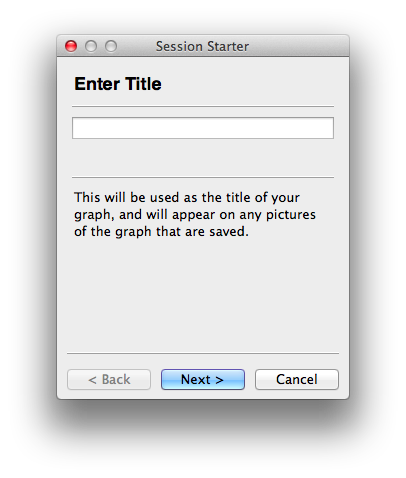
\includegraphics[width=\textwidth]{images/wizard_page_1.png}
        \caption{Wizard title chooser page}
        \label{fig:page_1}
    \end{subfigure}
    \begin{subfigure}[b]{0.24\textwidth}
        \centering
        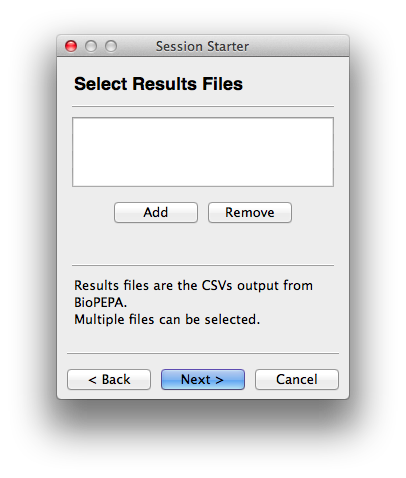
\includegraphics[width=\textwidth]{images/wizard_page_2.png}
        \caption{Wizard results selector page}
        \label{fig:page_2}
    \end{subfigure}

    \begin{subfigure}[b]{0.24\textwidth}
        \centering
        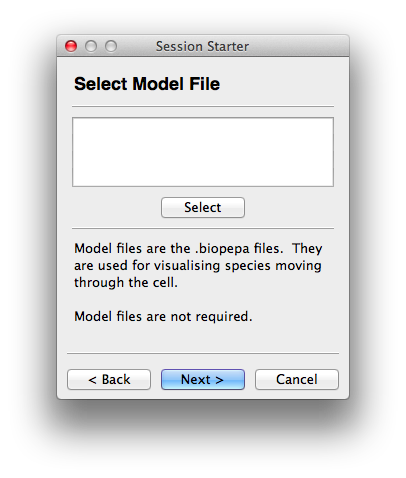
\includegraphics[width=\textwidth]{images/wizard_page_3.png}
        \caption{Wizard model selector page}
        \label{fig:page_3}
    \end{subfigure}
    \begin{subfigure}[b]{0.24\textwidth}
        \centering
        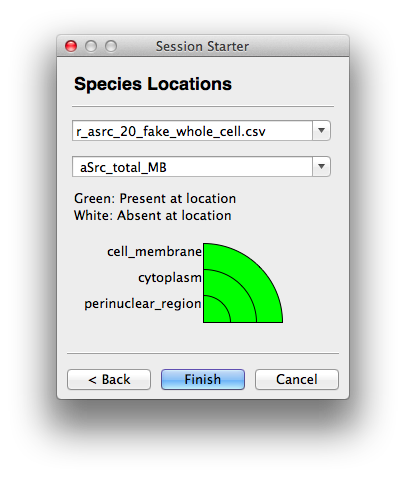
\includegraphics[width=\textwidth]{images/wizard_page_4.png}
        \caption{Wizard model viewing page}
        \label{fig:page_4}
    \end{subfigure}
    \caption{The session wizard that guides a user when setting up a session.}
    \label{fig:session_wizard}
\end{figure}

Form validators are used on the title fields and results fields.  The validators ensure that a title and at least one results file are included.  This stops the user from creating an invalid session.  There is also help text on each page of the wizard instructing the user on what actions they should take.

The model viewer page in Figure~\ref{fig:page_4} is similar to the cell cross-sections used in animation~\ref{sec:animation}.  There are two drop down boxes.  These drop down boxes control what is displayed in the cell cross-section.  Species in files can be selected.  The cell cross-section displays which compartments in the cell the species is present in.  The compartments are parsed from the model file.  This means that the model file is a requirement for model viewing and cell level animation.  This cell cross-section has replaced the previous model visualisation.  This model visualisation has two purposes. First, the user can sanity check that they have matching results and model files.  If a section of the cell has been left white then it acts as a cue to the user: if they were expecting the species to be present at that location then they know something has gone wrong.  Second, they can see how the model is structured.  The sections of the cell are labelled allowing the user to know what areas of the cell a species is present in.  This will hopefully increase their confidence with visualising and analysing the results from the models. Before the compartments were parsed from the model file automatically there was an user unfriendly system where the user had to input where in the cell a species is.  This was time consuming, difficult to use, and quite brittle.  At the time it assumed that there would be three compartments for every species, which is not a valid assumption.

\section{First Evaluation}

The first evaluation in the second phase of the project occurred in November 2014.  The user group was made up of two people.  One who had taken part in the first evaluation meeting and one person who had no knowledge of the project.

\subsection{User Group}

As I did not have a domain expert available I was not able to do insight based evaluation.  I took a more traditional approach.  Before the evaluation I prepared a typical scenario that a user might encounter.  The task was to open a file, annotate it and run the animation visualisation, and attach supporting documentation.  The task was prepared at two levels of instruction.  The first level was a paragraph of text that described what was to be done.  The second level was a step-by-step list of instructions to perform.  I observed the user group as they attempted the task and offered assistance when required.  Afterwards the user group was given a questionnaire to fill in about their experience. After filling in the questionnaire we went through and discussed their answers and any further thoughts that they had.

The task was prepared at two levels to try and gauge how easy the program is to use.  The users were first presented with the textual description and if they had been unable to complete the task with this then they would have been given the step-by-step instructions instead.  The users were able to complete the task from the textual description alone.  This is a good sign that the new tool is usable.

Some issues were encountered:

\begin{itemize}
\item The users were unfamiliar with MacOS -- Both users were unable to locate the menu bar as it is not attached to the program as in Windows.  Future evaluations will use Windows.
\item The users were unclear as to what was going to happen when annotating.  When annotating the graph with an arrow the user has to click twice to place it but there is no indication of this, nor was it clear to them which way the arrow would be drawn.  This has now been fixed. Different cursors are used to give feedback to the user that they should click, and rather than just relying on two clicks with no information as to where the arrow is going to point, after the first click (which places the tail of the arrow) an arrow will be drawn that follows the cursor until the second click placing the annotation.
\item Lack of ability to edit, move, or delete annotations -- Once an annotation was placed it was there permanently.  The ability to edit annotations was always planned, but had not been implemented in time.  But the amount of frustration it gave the users was very high.  It was a principle in all three of Norman, Neilson and Schniederman's lists that a user should be able to fix mistakes.  Since the evaluation, editing and deleting of annotations have been implemented.  This means any mistakes can be corrected.
\item Initially they were confused by what all the buttons on the matplotlib toolbar did.  After discovering the tooltips and seeing what effect the buttons had they were comfortable with them.  If a user were to do something they did not intend they are able to undo it. All the matplotlib built-in buttons on the toolbar can be undone and redone from the toolbar.  Any buttons implemented for this tool are covered by the undo and redo functionality implemented across the whole program.  Being able to recover from their actions on the toolbar means no hindrance to discovery and so needs no further action.  It would be desirable to have the two undo methods unified but a way to do this could not be found.
\item The users were confused by some of the terminology.  In particular ``save graph'' and ``save model''. These items in the menu have now been grouped more carefully to help the user distinguish them.  A related issue was worrying that ``save graph'' was going to override the results file.  To rectify this the menu items that create new files have been renamed ``export ...''.
\item The users struggled to start a new session.  When asked for a title they did not know what the title was going to be used for.  When trying to add files, rather than use the add files button in the dialogue, they tried to use the file menu.  Having two routes into the visualisation seemed to be confusing them.  Now the file menu open file has been removed.  To create a visualisation the user has to go through the new session wizard.
\item When placing species in the cell one of the users did not understand what they were being asked to do.  One of the users did understand.  To fix this user input has been removed from the equation.  This has required the model file to also be chosen, but then species locations are parsed automatically.
\item They liked the animation feature and thought it would be very useful (One of the users did their PhD in transport and expressed a desire to have had this feature during the PhD).  They did feel that it wouldn't be useful directly for papers, but that it would be useful when deciding what to include in a paper.
\item One of the users asked if there was a map of the cell.  When presented with the model visualisation they thought that it did look nice, but they were unsure of its usefulness.  The model viewing has since been merged into the animation visualisation.
\item The results from the questionnaire indicated that both users thought the tool's appearance was good.  The tool was average in difficulty to use -- neither easy nor difficult. The annotation buttons on the toolbar were clear as to what they did. It was obvious how to attach supporting files.  Both users thought that it is very useful to attach files to the session so that they can be easily emailed to a colleague.  They thought it would be useful to have the graph automatically annotated, but they wanted to the ability to disable any automatic annotations.  Both users found the animation useful.
\end{itemize}

\subsection{Personal}

\tdi{probably needs a big going over}

At this stage in the development the program was in a state where some existing functionality had been broken and gone unnoticed during the implementation of the new features.  This highlighted architectural flaws in the code.  There were multiple paths through the program that data was taking, and duplicated code in places.  Since then a majority of these bugs have been ironed out and the duplications removed. The code much better architected.  At the time of the evaluation with the users not all the features could be tested with them -- mainly the plot preferences dialogue.  These features have now been fixed and they will be evaluated by the users at the next meeting.

Having the users use the program has also highlighted a number of usability problems: menus being badly organised and named, features such as annotation rely on assumed knowledge to work them.  All this created an unfriendly environment for the user.  This was due to losing sight of the need for usability during development and when testing new features not removing the knowledge of the code from my mind.  Since this evaluation the three lists of usability have been refocused on and the code gone through and the principles applied.

I am pleased with the positive feedback on animation and annotation -- two of the core new features.

\section{Evaluation 2 - Start of Second Semester}
\subsection{User Group}

\tdi{do it like above}

\subsection{Personal}

\subsection{vashti}

\tdi{do it like above}

\section{Evaluation 3 - End of Second Semester}
\subsection{User Group}
\subsection{Expert User}

\tdi{why not happening }

\tdi{vashti}

\subsection{Personal}

\section{Overall Self Evaluation}
Scribble over lots of stuff talk about changes

\tdi{final ui}

\tdi{talk about the architecture}
\tdi{talk about perhaps being more strictly mvc}
\tdi{evaluate the evaluation strategy}

\tdi{evaluate collaboration}

\subsection{Search Results}
\tdi{move this into evaluation?}
Initial results are very promising with the tf.idf weighted cosine providing much clearer results than with simple euclidean distance.  There is not a large enough truth set of plot similarities to be able to confidently say that it is effective.  However these early promising results seem to indicate that further research would certainly be worthwhile, but outside the scope of the project.
